\makeheading{Lecture 6 | 2020-09-20}
\underline{Author's note}: Diagrams will be omitted for most of the text,
unless the example is not trivial. Students are encouraged
to draw the diagrams when following the examples.
\begin{Example}{}{}
    Let $ X $ and $ Y $ be continuous random variables
    with joint p.d.f.\
    \[ f(x,y)=
        \begin{cases}
            x+y & 0\le x\le 1,\quad 0\le y\le 1 \\
            0   & \text{otherwise}
        \end{cases} \]
    \begin{enumerate}[label=(\roman*)]
        \item Show $ f(x,y) $ is a joint p.d.f.\
        \item Find
              \begin{enumerate}[label=(\alph*)]
                  \item $ \Prob{X\le 1/3, Y\le 1/2} $
                  \item $ \Prob{X\le Y} $
                  \item $ \Prob{X+Y\le 1/2} $
                  \item $ \Prob{XY\le 1/2} $
              \end{enumerate}
        \item Find marginal p.d.f.\ of $ X $ and $ Y $.
    \end{enumerate}
    \textbf{Solution.}
    \begin{enumerate}[label=(\roman*)]
        \item Note that $ f(x,y)\ge 0 $. We need to show
              \[ \int_{-\infty}^{\infty} \int_{-\infty}^{\infty} f(x,y)\, d{y} \, d{x} =1 \]
              \begin{align*}
                  \int_{-\infty}^{\infty} \int_{-\infty}^{\infty} f(x,y)\, d{y} \, d{x}
                   & =\int_{0}^{1} \int_{0}^{1} (x+y)\, d{y} \, d{x}         \\
                   & =\int_{0}^{1} \left[ x+\frac{y^2}{2} \right]_0^1\, d{x} \\
                   & =\int_{0}^{1} \left( x+\frac{1}{2} \right)\, d{x}       \\
                   & =\left[ \frac{x^2}{2}  +\frac{x}{2}\right]_0^1          \\
                   & =1
              \end{align*}
        \item \begin{enumerate}[label=(\alph*)]
                  \item Take $ R=\set{(x,y):0\le x\le 1/3, 0\le y
                                \le 1/2} $.
                        \begin{align*}
                            \int_{0}^{1/3} \int_{0}^{1/2} (x+y)\, d{y} \, d{x}
                             & =\int_{0}^{1/3}
                            \left[ xy +\frac{y^2}{2}  \right]_0^{1/2}\, d{x}                  \\
                             & =\int_{0}^{1/3} \left( \frac{x}{2} +\frac{1}{8} \right)\, d{x} \\
                             & =\left[ \frac{x^2}{4}+\frac{x}{8} \right]_0^{1/3}              \\
                             & =\frac{1}{36}+\frac{1}{24}                                     \\
                             & =\frac{5}{72}
                        \end{align*}
                  \item $ R=\set{(x,y):0\le x\le 1,x\le y\le 1} $.
                        \begin{align*}
                            \int_{0}^{1} \int_{x}^{1} (x+y)\, d{y} \, d{x}
                             & =\int_{0}^{1} \left[ xy +\frac{y^2}{2}  \right]_x^1 \, d{x} \\
                             & =\int_{0}^{1} x+\frac{1}{2}-x^2-\frac{x^2}{2}\, d{x}        \\
                             & =\left[ \frac{x^2}{2} +\frac{x}{2} -\frac{x^3}{3}-
                            \frac{x^3}{2}\left( \frac{1}{3} \right)  \right]_0^1           \\
                             & =\frac{1}{2}
                        \end{align*}
                  \item $ R=\set{(x,y):0\le x\le
                                1/2,0\le y\le (1/2)-x } $
                        \begin{align*}
                            \int_{0}^{1/2} \int_{0}^{(1/2)-x} (x+y)\, d{y} \, d{x}
                             & =\int_{0}^{1/2} \left[ xy+\frac{y^2}{2} \right]_{0}^{(1/2)-x}\, d{x}           \\
                             & =\int_{0}^{1/2} \left( \frac{x}{2} -x^2+\frac{1}{8}
                            -\frac{x}{2} +\frac{x^2}{2}   \right)\, d{x}                                      \\
                             & =\int_{0}^{1/2} \frac{1}{8} -\frac{x^2}{2}\, d{x}                              \\
                             & =\left[ \frac{x}{8} -\frac{x^3}{2} \left( \frac{1}{3}  \right) \right]_0^{1/2} \\
                             & =\frac{1}{24}
                        \end{align*}
                  \item This example is a bit complicated,
                        so I included a figure.
                        \begin{center}
                            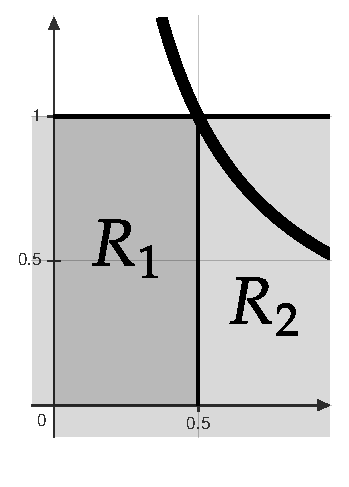
\includegraphics[width=0.6\textwidth]{fig2.pdf}
                        \end{center}
                        Note the curve drawn is $ xy=1/2 $.
                        $ R_1 $ can be described with:
                        \[ 0\le x\le \frac{1}{2}   \]
                        \[ 0\le y\le 1 \]
                        $ R_2 $ (region below the curve) can be described with:
                        \[ \frac{1}{2} \le x\le 1 \]
                        \[ 0\le y\le \left( \frac{1}{2} \right)/x  \]
                        Therefore, we need to evaluate two double integrals.
                        \begin{align*}
                            \int_{0}^{1/2} \int_{0}^{1} (x+y)\, d{y} \, d{x}
                            +\int_{1/2}^{1} \int_{0}^{(1/2)/x} (x+y)\, d{y} \, d{x}=\frac{3}{4} \\
                        \end{align*}
              \end{enumerate}
        \item The support of $ X $ is $ \interval{0}{1} $.
              \[ f_1(x)=0\iff x<0\text{ or } x>1 \]
              Therefore, we focus on $ 0\le x\le 1 $.
              \[ f_1(x)=\int_{-\infty}^{\infty} f(x,y)\, d{y}
                  =\int_{0}^{1} (x+y)\, d{y}=\left[ x+\frac{y^2}{2} \right]_0^1
                  =x+\frac{1}{2} \]
              Thus,
              \[ f_1(x)=
                  \begin{dcases}
                      x+\frac{1}{2} & 0\le x\le 1      \\
                      0             & \text{otherwise}
                  \end{dcases} \]
              $ f_2(y) $ is similar by symmetry.
    \end{enumerate}
\end{Example}
\begin{Example}{}{}
    Suppose
    \[ f(x,y)=\begin{dcases}
            ke^{-x-y} & 0<x<y<\infty     \\
            0         & \text{otherwise}
        \end{dcases} \]
    is the joint p.d.f.\ of $ (X,Y) $.
    \begin{enumerate}[label=(\roman*)]
        \item Find $ k $.
        \item Find
              \begin{enumerate}[label=(\alph*)]
                  \item $ \Prob{X\le 1/3,Y\le 1/2} $
                  \item $ \Prob{X\le Y} $
                  \item $ \Prob{X+Y\ge 1} $
              \end{enumerate}
        \item Marginal p.d.f.\ of $ X $ and $ Y $.
        \item Suppose $ T=X+Y $, find the p.d.f.\ of $ T $.
    \end{enumerate}
    \textbf{Solution.}
    \begin{enumerate}[label=(\roman*)]
        \item We know $ f(x,y)\ge 0\iff k\ge 0 $. Actually,
              $ k>0 $ since if $ k=0 $, then $ f(x,y)\equiv 0 $.
              We solve $ k $ by solving the following:
              \[ \int_{-\infty}^{\infty} \int_{-\infty}^{\infty} f(x,y)\, d{x} \, d{y} =1 \]
              Therefore,
              \begin{align*}
                   & =\int_{0}^{\infty} \int_{x}^{\infty} ke^{-x-y}\, d{y} \, d{x}     \\
                   & =k \int_{0}^{\infty} e^{-x}\left[ -e^{-y} \right]_x^\infty\, d{x} \\
                   & =k \int_{0}^{\infty} e^{-x}e^{-x}\, d{x}                          \\
                   & =k \int_{0}^{\infty} e^{-2x}\, d{x}                               \\
                   & =k\left[ -\frac{1}{2} e^{-2x} \right]_0^\infty                    \\
                   & =\frac{k}{2}
              \end{align*}

              Thus, $ k/2=1\implies k=2 $.
        \item \begin{enumerate}[label=(\alph*)]
                  \item $ \Prob{X\le 1/3,Y\le 1/2} $.
                        \[ R=\set{(x,y):0\le x\le 1/3, x\le y\le 1/2} \]
                        Therefore,
                        \begin{align*}
                            \Prob{X\le 1/3,Y\le 1/2}
                             & =\int_{0}^{1/3} \int_{x}^{1/2} 2e^{-x-y}\, d{y} \, d{x}                                              \\
                             & =2\int_{0}^{1/3} e^{-x}\left[ -e^{-y} \right]_x^{1/2}\, d{x}                                         \\
                             & =2 \int_{0}^{1/3} e^{-x}\left( -e^{-1/2}+e^{-x} \right)\, d{x}                                       \\
                             & =2 \int_{0}^{1/3} -e^{-1/2}e^{-x}+e^{-2x}\, d{x}                                                     \\
                             & =2\left( -e^{-1/2}\left[ -e^{-x} \right]_0^{1/3}+\left[ -\frac{1}{2} e^{-2x} \right]_0^{1/3} \right) \\
                             & =2\left( -e^{-1/2}\left( -e^{-1/3}+1 \right)+\left( -\frac{1}{2}  \right)
                            \left( e^{-2/3}-1 \right) \right)                                                                       \\
                             & =2\left(1/2+e^{-5/6}-e^{-1/2}-\frac{1}{2}e^{-2/3}\right)                                             \\
                             & =1-e^{-2/3}+2\left(e^{-5/6}-e^{-1/2}\right)                                                          \\
                             & \approx 0.1427
                        \end{align*}
                  \item $ \Prob{X\le Y} $. Note that the region
                        is the same as the support. Therefore,
                        \[ \Prob{X\le Y}
                            =\iint\limits_{x\le y}f(x,y)dx\,dy=1 \]
                  \item $ \Prob{X+Y\ge 1} $. Note that this region is a
                        bit complicated, so we will consider $ 1-\Prob{X+Y<1}
                            =1-\Prob{X+Y\le 1} $.
                        The equal sign does not account for any area (it's continuous,
                        but not required to know in this course).
                        \[ R=\set{(x,y):0\le x\le 1/2,x\le y\le 1-x} \]
                        \begin{align*}
                            \Prob{X+Y\le 1}
                             & =\int_{0}^{1/2} \int_{x}^{1-x} 2e^{-x}e^{-y}\, d{y} \, d{x}         \\
                             & =2\int_{0}^{1/2} e^{-x}\left[ e^{-y} \right]_{x}^{1-x}\, d{x}       \\
                             & =2 \int_{0}^{1/2} e^{-x}\left( -e^{x-1}+e^{-x} \right)\, d{x}       \\
                             & =2 \int_{0}^{1/2} -e^{-1}+e^{-2x}\, d{x}                            \\
                             & =2 \left[ -xe^{-1}-\frac{1}{2} e^{-2x} \right]_0^{1/2}              \\
                             & =2\left( \left( -\frac{1}{2} e^{-1}-\frac{1}{2} e^{-2(1/2)} \right)
                            -\left( 0-\frac{1}{2} \right) \right)                                  \\
                             & =2\left( -\frac{1}{2} e^{-1}-\frac{1}{2} e^{-1}+\frac{1}{2}
                            \right)                                                                \\
                             & =2\left( -e^{-1}+\frac{1}{2} \right)                                \\
                             & =1-2e^{-1}
                        \end{align*}
                        Thus, $ \Prob{X+Y\ge 1}
                            =1-\Prob{X+Y\le 1}
                            =1-\left( 1-2e^{-1} \right)=2e^{-1} $.
              \end{enumerate}
        \item Marginal p.d.f.\ of $ X $. The support of $ X $ is
              $ \interval[open]{0}{\infty} $. We know $ x>0 $, so
              \[ f_1(x)=
                  \int_{-\infty}^{\infty} f(x,y)\, d{y}
                  =\int_{x}^{\infty} 2e^{-x-y}\, d{y}
                  =2e^{-x}\left[ -e^{-y} \right]_x^\infty=2e^{-2x} \]
              The marginal p.d.f.\ of $ Y $. The support of $ Y $ is
              $ \interval[open]{0}{\infty} $. We know $ y>0 $, so
              \[ f_2(y)=
                  \int_{0}^{y}2e^{-x-y}\, d{x} =
                  2e^{-y}\left[ -e^{-x} \right]_0^y
                  =2e^{-y}\left( 1-e^{-y} \right)=
                  2e^{-y}-2e^{-2y} \]
        \item Suppose $ T=X+Y $, find the p.d.f.\ of $ T $.
              We first find the c.d.f.\ of $ T $, then we take the derivative
              of $ T $.

              Support of $ T $ is $ \interval[open]{0}{\infty} $.

              When $ t\le 0 $, $ F_T(t)=\Prob{T\le t}=0 $,
              so we only focus on $ t>0 $, so $ F_T(t)=\Prob{T\le t} $.
              \[ R=\set{(x,y):0\le x\le t/2, x\le y\le t-x} \]
              Therefore,
              \begin{align*}
                  F_T(t)
                   & = \int_{0}^{t/2} \int_{x}^{t-x} 2e^{-x-y}\, d{y} \, d{x}             \\
                   & =2 \int_{0}^{t/2} e^{-x}\left[ -e^{-y} \right]_x^{t-x}\, d{x}        \\
                   & =2 \int_{0}^{t/2} e^{-x}\left( -e^{x-t}+e^{-x} \right)\, d{x}        \\
                   & =2 \int_{0}^{t/2} -e^{-t}+e^{-2x}\, d{x}                             \\
                   & =2\left[ -xe^{-t}-\frac{1}{2}e^{-2x} \right]_0^{t/2}                 \\
                   & =2\left( \left( -\frac{t}{2} e^{-t} -\frac{1}{2} e^{-t}\right)
                  -\left( 0-\frac{1}{2}  \right) \right)                                  \\
                   & =2\left( -\frac{t}{2} e^{-t}-\frac{1}{2} e^{-t}+\frac{1}{2}  \right) \\
                   & =1-e^{-t}-te^{-t}
              \end{align*}
              So,
              \[ F_T(t)=
                  \begin{dcases}
                      1-e^{-t}-te^{-t} & t>0    \\
                      0                & t\le 0
                  \end{dcases} \]
              Therefore, by computing $ \displaystyle
                  \frac{d}{dt}[F_T(t)] $, the p.d.f.\ of $ T $ is
              \[ f_T(t)=
                  \begin{dcases}
                      te^{-t} & t> 0   \\
                      0       & t\le 0
                  \end{dcases} \]
    \end{enumerate}
\end{Example}
